\documentclass{beamer}
\usetheme{Madrid}

\usepackage{amsmath, amssymb, amsthm}
\usepackage{graphicx}
\usepackage{gensymb}
\usepackage[utf8]{inputenc}
\usepackage{hyperref}
\usepackage{tikz}


\title{4.4.8 Matgeo}
\author{AI25BTECH11012 - Garige Unnathi}
\date{}

\begin{document}

\frame{\titlepage}

% Question frame
\begin{frame}
\frametitle{Question}
Find the value of x such that the four points A(x,5,-1), B(3,2,1), C(4,5,5), and
D(4,2,-2) are coplanar.\\
\end{frame}


% Solution steps
\begin{frame}
\frametitle{Solution}
The equation of a plane can be given by the formula :
         
\begin{align}
    n^{T}\textbf{x} = 1\\
    or\\
    x^{T}\textbf{n} =1 
\end{align}

Since all the points A,B,C,D are on the plane :
\begin{align}
   A^{T}n =1 \quad  B^{T}n =1 \quad  C^{T}n =1 \quad  D^{T}n =1 
\end{align}


\end{frame}



\begin{frame}
\frametitle{Solution}
To find \textbf{D} we find \textbf{n} :\\
Combining the above equation we get :


\begin{align}
   \begin{bmatrix}B \\ C \\ D\end{bmatrix}^{T}\textbf{n}  = \begin{bmatrix}3 & 2 & 1\\
                                     4 & 5  &  5 \\
                                     4 & 2 &-2\end{bmatrix}\textbf{n}  = \begin{bmatrix}1\\1\\1\end{bmatrix}
\end{align}
solving the equation by row reduction we get 
\begin{align}
     \textbf{n} =  \begin{bmatrix}\frac{9}{16} \\ -\frac{7}{16} \\ \frac{3}{16}\end{bmatrix} = \frac{1}{16} \begin{bmatrix}9 \\ -7 \\ 3\end{bmatrix}
\end{align}
\end{frame}

\begin{frame}
\frametitle{Solution}
substituting in the equation $A^{T}n =1 $ we get:

\begin{align}
    \begin{bmatrix}x & 5 &-1\end{bmatrix}\begin{bmatrix}9\\-7\\3\end{bmatrix} = 16\\
    9x - 35 - 3 = 16 \\
    9x = 54
\end{align}
\begin{align}
    x = 6
\end{align}

\end{frame}

% Graphical representation
\begin{frame}

\frametitle{Graphical Representation}
\begin{center}
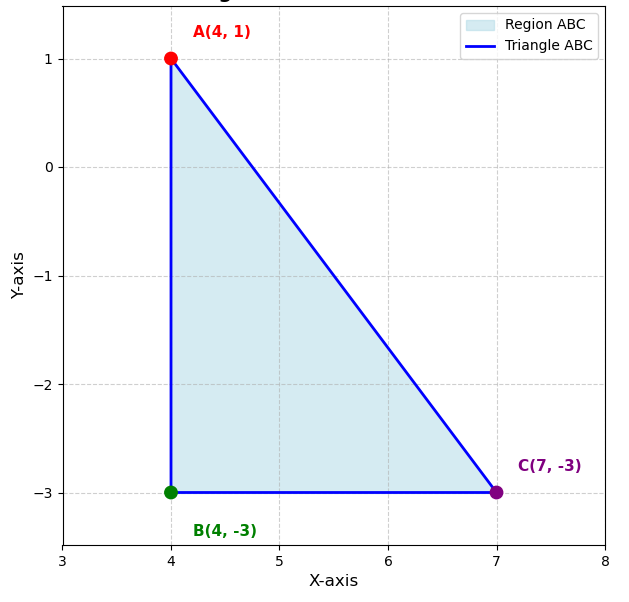
\includegraphics[width=0.6\linewidth]{/Users/unnathi/Documents/ee1030-2025/ai25btech11012/matgeo/4.4.8/figs/fig.png}
\end{center}
\end{frame}

\end{document}
